% EN49 c10 | 原书 p.98–111（PDF 109–122） | 第 7 章 §7.1–7.2
% 每页起首用 % ===== 原书 p.N ===== 注释标记。

\section{粘合图表}

\subsection{扇形粘合}

% ===== 原书 p.98 =====
本节的主要结果将利用 §2 的构造，给出补集 $(\C^*)^n\setminus H$ 的一个扇形分解。

\begin{proposition}\label{prop:7-1-1}
Liouville 流形 $(\C^*)^n\setminus H$ 简单 Liouville 同伦于 $(H\times\C^*,z)$ 沿 $H$ 到 $((\C^*)^n,f)$ 的扇形粘合。
\end{proposition}

\begin{proof}
如前所述，对 $F_{R_1}\cap\{\phi\le R_2\}$ 应用 [Syl19b, Prop 2.6]，并在 [Syl19b] 所说明的小形变之后，得到形如
\[
U=\bigl(H\times\{z\in\C:\operatorname{Re}(z)>-\rho\},\ \lambda_{(\C^*)^n}|_F+\lambda_\C^{\operatorname{std}}\bigr)
\]
的标准 Liouville 邻域 $U$。

% ===== 原书 p.99 =====
\begin{figure}[htbp]
\centering
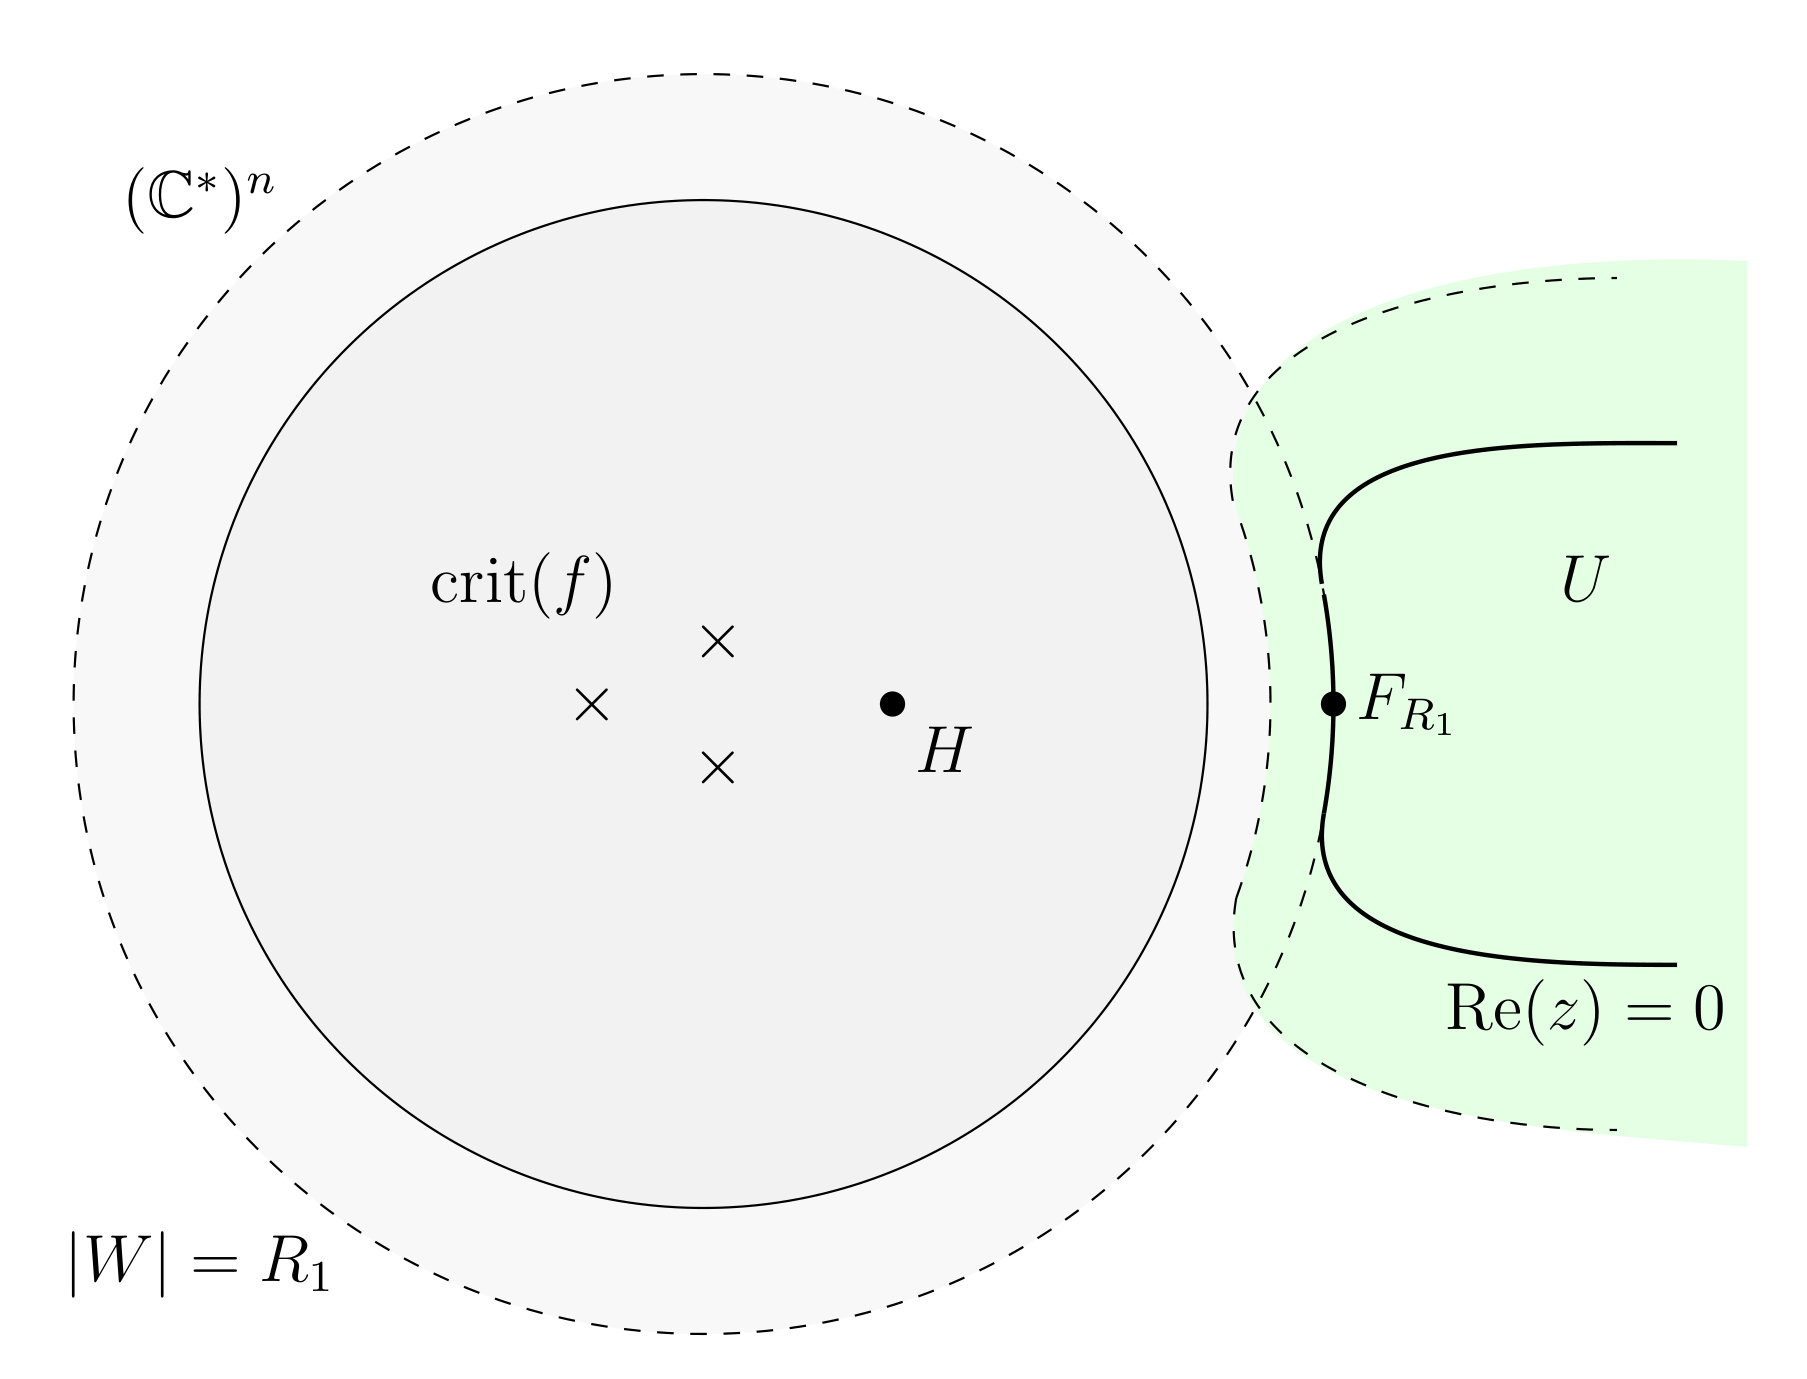
\includegraphics[width=0.56\textwidth]{figures/fig7_1.png}
\caption{命题 \ref{prop:7-1-1} 的证明：$U$（绿色）是纤维 $F_{R_1}$（黑点）的乘积邻域。}
\label{fig:7-1}
\end{figure}

$U$ 在完备化 $(\C^*)^n$ 中真嵌入。这里我们重申 $F_{R_1}$ 与 $H$ 的等同方式：沿一条射线作平行移动。于是扇形超曲面 $\{\operatorname{Re}(z)=0\}$ 把 $(\C^*)^n$ 表示成沿 $H$ 把 $(H\times\C,z)$ 粘到 $((\C^*)^n,f)$ 的扇形粘合（见图 \ref{fig:7-1}）。

接下来，我们在 $H\times\{z\in\C:\operatorname{Re}(z)>-\rho\}\setminus\{\rho\}$ 上引入一个 Liouville 形式，使它与原 Liouville 形式之差支撑在 $H\times\{\rho\}$ 的一个小开邻域上，做法如 [Jef22, Proposition 6]。此时超曲面 $\{\operatorname{Re}(z)=0\}$ 在无穷远处仍平行于 Liouville 向量场，于是可以把 $H\times\{z\in\C:\operatorname{Re}(z)>-\rho\}\setminus\{\rho\}$ 沿 $H$ 粘回一个与 $((\C^*)^n,f)$ 典范等同的扇形。另一方面，$(\C^*)^n$ 内存在 Liouville 超曲面的同痕，把 $H\times\{\rho\}$ 移到 $f^{-1}(0)$。

% ===== 原书 p.100 =====
\begin{figure}[htbp]
\centering
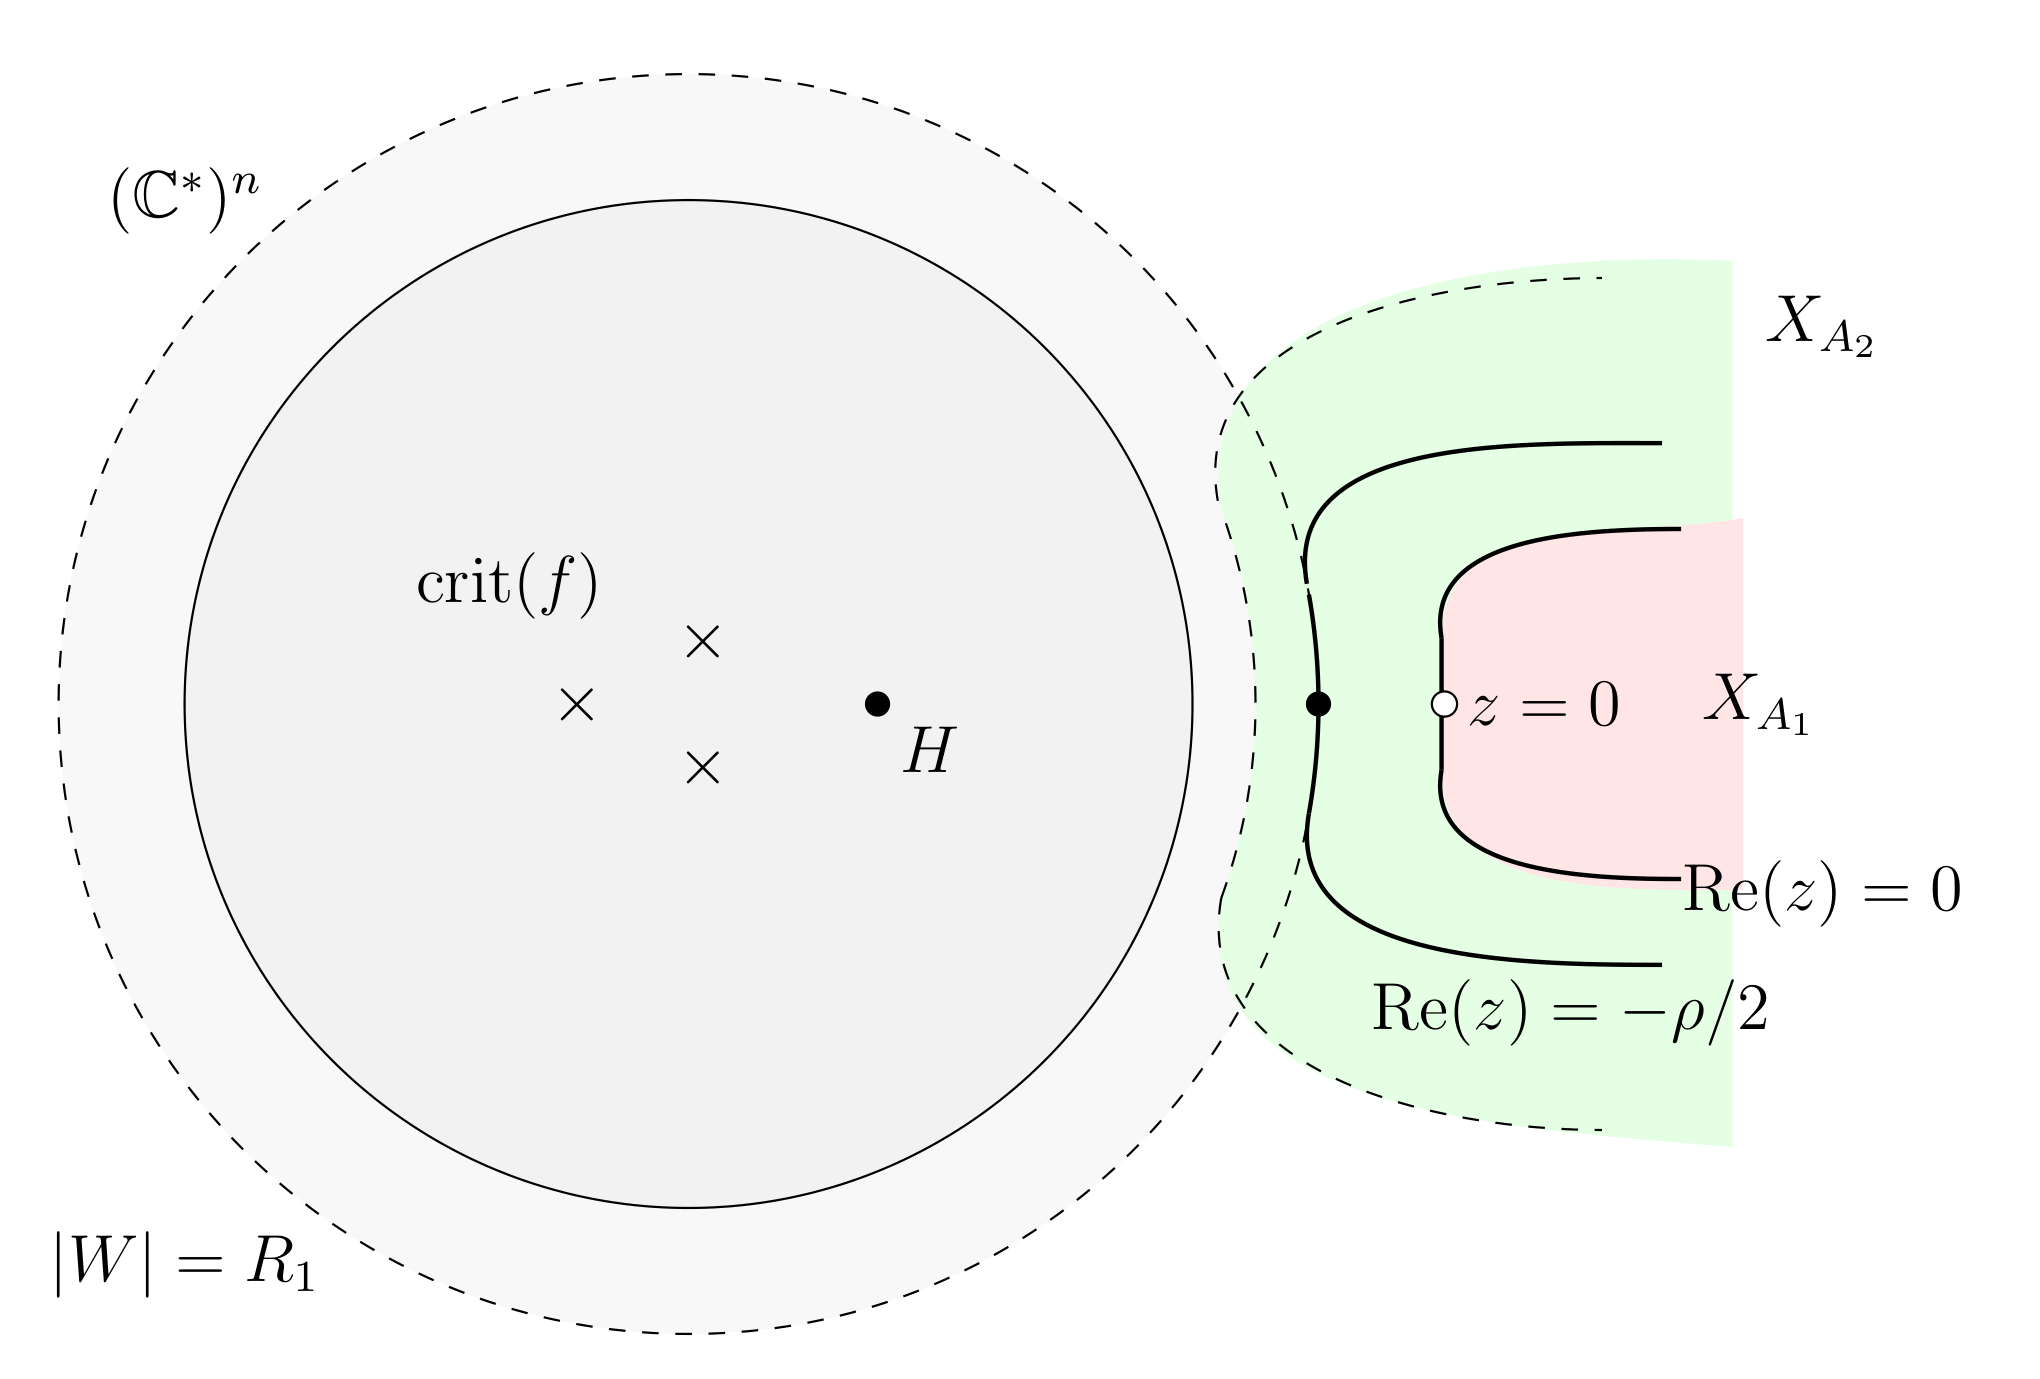
\includegraphics[width=0.64\textwidth]{figures/fig7_2.png}
\caption{命题 \ref{prop:7-1-2} 的证明：$X_{A_2}$ 为绿色，$X_{A_1}$ 为红色。}
\label{fig:7-2}
\end{figure}

于是应用 Moser 引理可知，这一粘合的结果与 $(\C^*)^n\setminus H$ 上的 Liouville 形式之间存在简单 Liouville 同伦；后者如 [Jef22] 所述，又与由限制得到的 $(\C^*)^n\setminus H\subseteq(\C^*)^{n+1}$ 上的原 Liouville 形式简单 Liouville 同伦。这就说明：沿 $H$ 把 $(H\times\C^*,z)$ 粘到 $((\C^*)^n,f)$ 所得的结果，同伦之后正是 $(\C^*)^n\setminus H$：见图 \ref{fig:7-2}。
\end{proof}

\transnote{易错预警：$F_{R_1}$ 与 $H$ 的等同依赖“沿一条射线作平行移动”这一选择，换一条射线会给出不同的等同；后文所有粘合映射都相对于这个选择。}

\transnote{含糊点拨：此处的 $z$ 是邻域 $U$ 上的坐标，它与原来的映射 $f$ 并不同；$z$ 的纤维只与 $f$ 的纤维同痕。原书在 p.99 明言这一点，读图 \ref{fig:7-1} 时容易误以为 $z=f$。}

\begin{remarkx}\label{rem:9}
我们应把这一分解看成与表示 $\tilde f_0=0$ 相联系的 $(\C^*)^n\setminus H$ 的扇形分解。
\end{remarkx}

\transnote{易错预警：$\tilde f_0$ 不是 $f$ 本身，而是 §2 中把 $0$ 处的单值性整理到无穷远之后得到的函数；两种表示 $\tilde f_0=0$ 与 $\tilde f_\infty=0$ 对应同一个 $(\C^*)^n\setminus H$，但扇形分解不同。}

回忆 [GPS19] 中的 $A_n$ 扇形：其定义是沿边界带 $n+1$ 个停点的标准 Liouville 圆盘 $D^2$。

\begin{proposition}\label{prop:7-1-2}
Liouville 流形 $(\C^*)^n\setminus H$ 简单 Liouville 同伦于如下扇形粘合：沿一条纤维 $H$ 把 $((\C^*)^n,f)$ 粘到扇形 $(E,H)$，而 $(E,H)$ 由 $H\times A_2$ 与 $H\times A_1$ 沿两个边界分支、通过等同 $\id\colon H\to H$ 与 $\mu\colon H\to H$ 粘合给出。
\end{proposition}

% ===== 原书 p.101 =====
\begin{figure}[htbp]
\centering
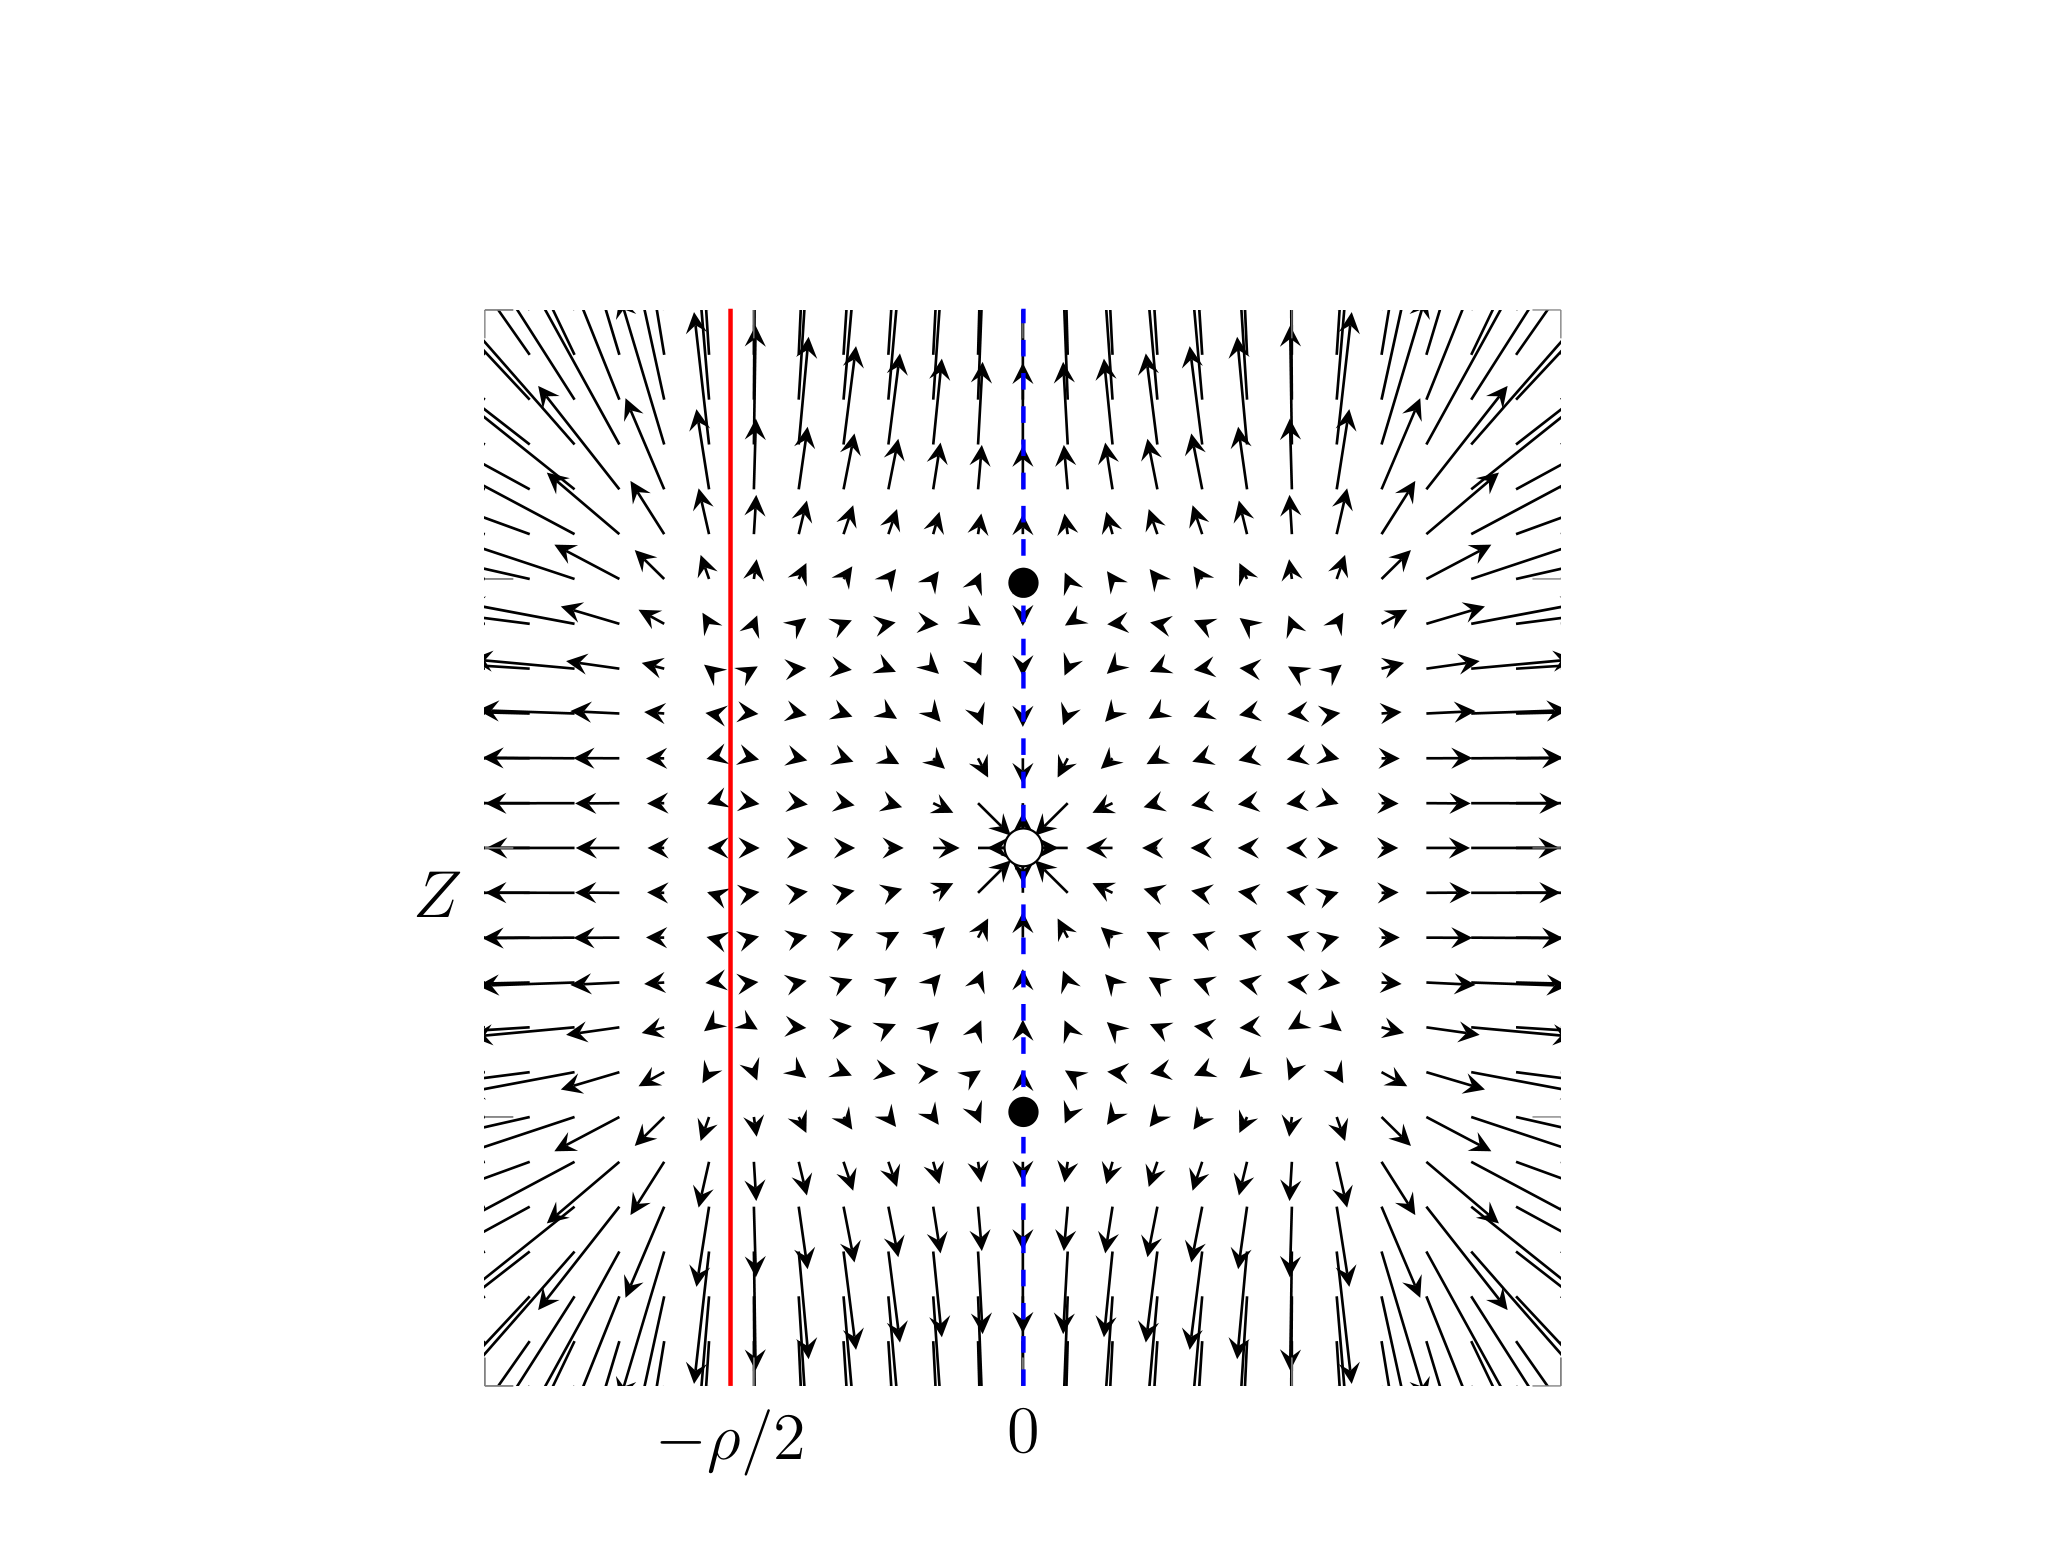
\includegraphics[width=0.52\textwidth]{figures/fig7_3.png}
\caption{命题 \ref{prop:7-1-2} 证明中形变后的 Liouville 向量场草图：超曲面 $\operatorname{Re}(z)=-\rho/2$ 为红色，两个黑点是 Liouville 向量场的零点。}
\label{fig:7-3}
\end{figure}

\begin{proof}
我们把证明拆成四步。先指出：若假定 $f$ 诱导出 $(\C^*)^n$ 边界的一个开书分解（open book decomposition），如 [GPS20a, Example 2.20] 所设，则论证可以大为简化。读者也可对照 [Gam20, Proposition 3.7]。

\transnote{含糊点拨：原文把“开书分解”当作可使论证大幅简化的额外假设，而未假定它成立；本证明不使用开书分解，只把这一情形作为对照。}

\begin{enumerate}
\item 设想延续上文命题 \ref{prop:7-1-1} 的论证：在邻域 $H\times\{z\in\C:\operatorname{Re}(z)>-\rho\}\setminus\{0\}$ 上存在显式的 Liouville 结构简单同伦，使 $\{\operatorname{Re}(z)=0\}$ 与 $\{\operatorname{Re}(z)=-\rho/2\}$ 都在无穷远处平行于 Liouville 向量场，并且仍以 $I=\operatorname{Im}(z)$ 作为 $I$-函数。所得 Liouville 向量场 $Z$ 的草图见图 \ref{fig:7-3}：它在 $\C^*$ 上处处有正散度，因而在彼处定义一个 Liouville 形式。这把 $(\C^*)^n\setminus H$ 表示成 $((\C^*)^n,f)$ 到两个扇形 $X_{A_2}\cong H\times A_2$ 与 $X_{A_1}\cong H\times A_1$ 的扇形粘合，粘合沿边界分支 $\partial(X_{A_2})$（它同痕于 $H\times\R$）进行（见图 \ref{fig:7-2}）。

% ===== 原书 p.102 =====
\begin{figure}[htbp]
\centering
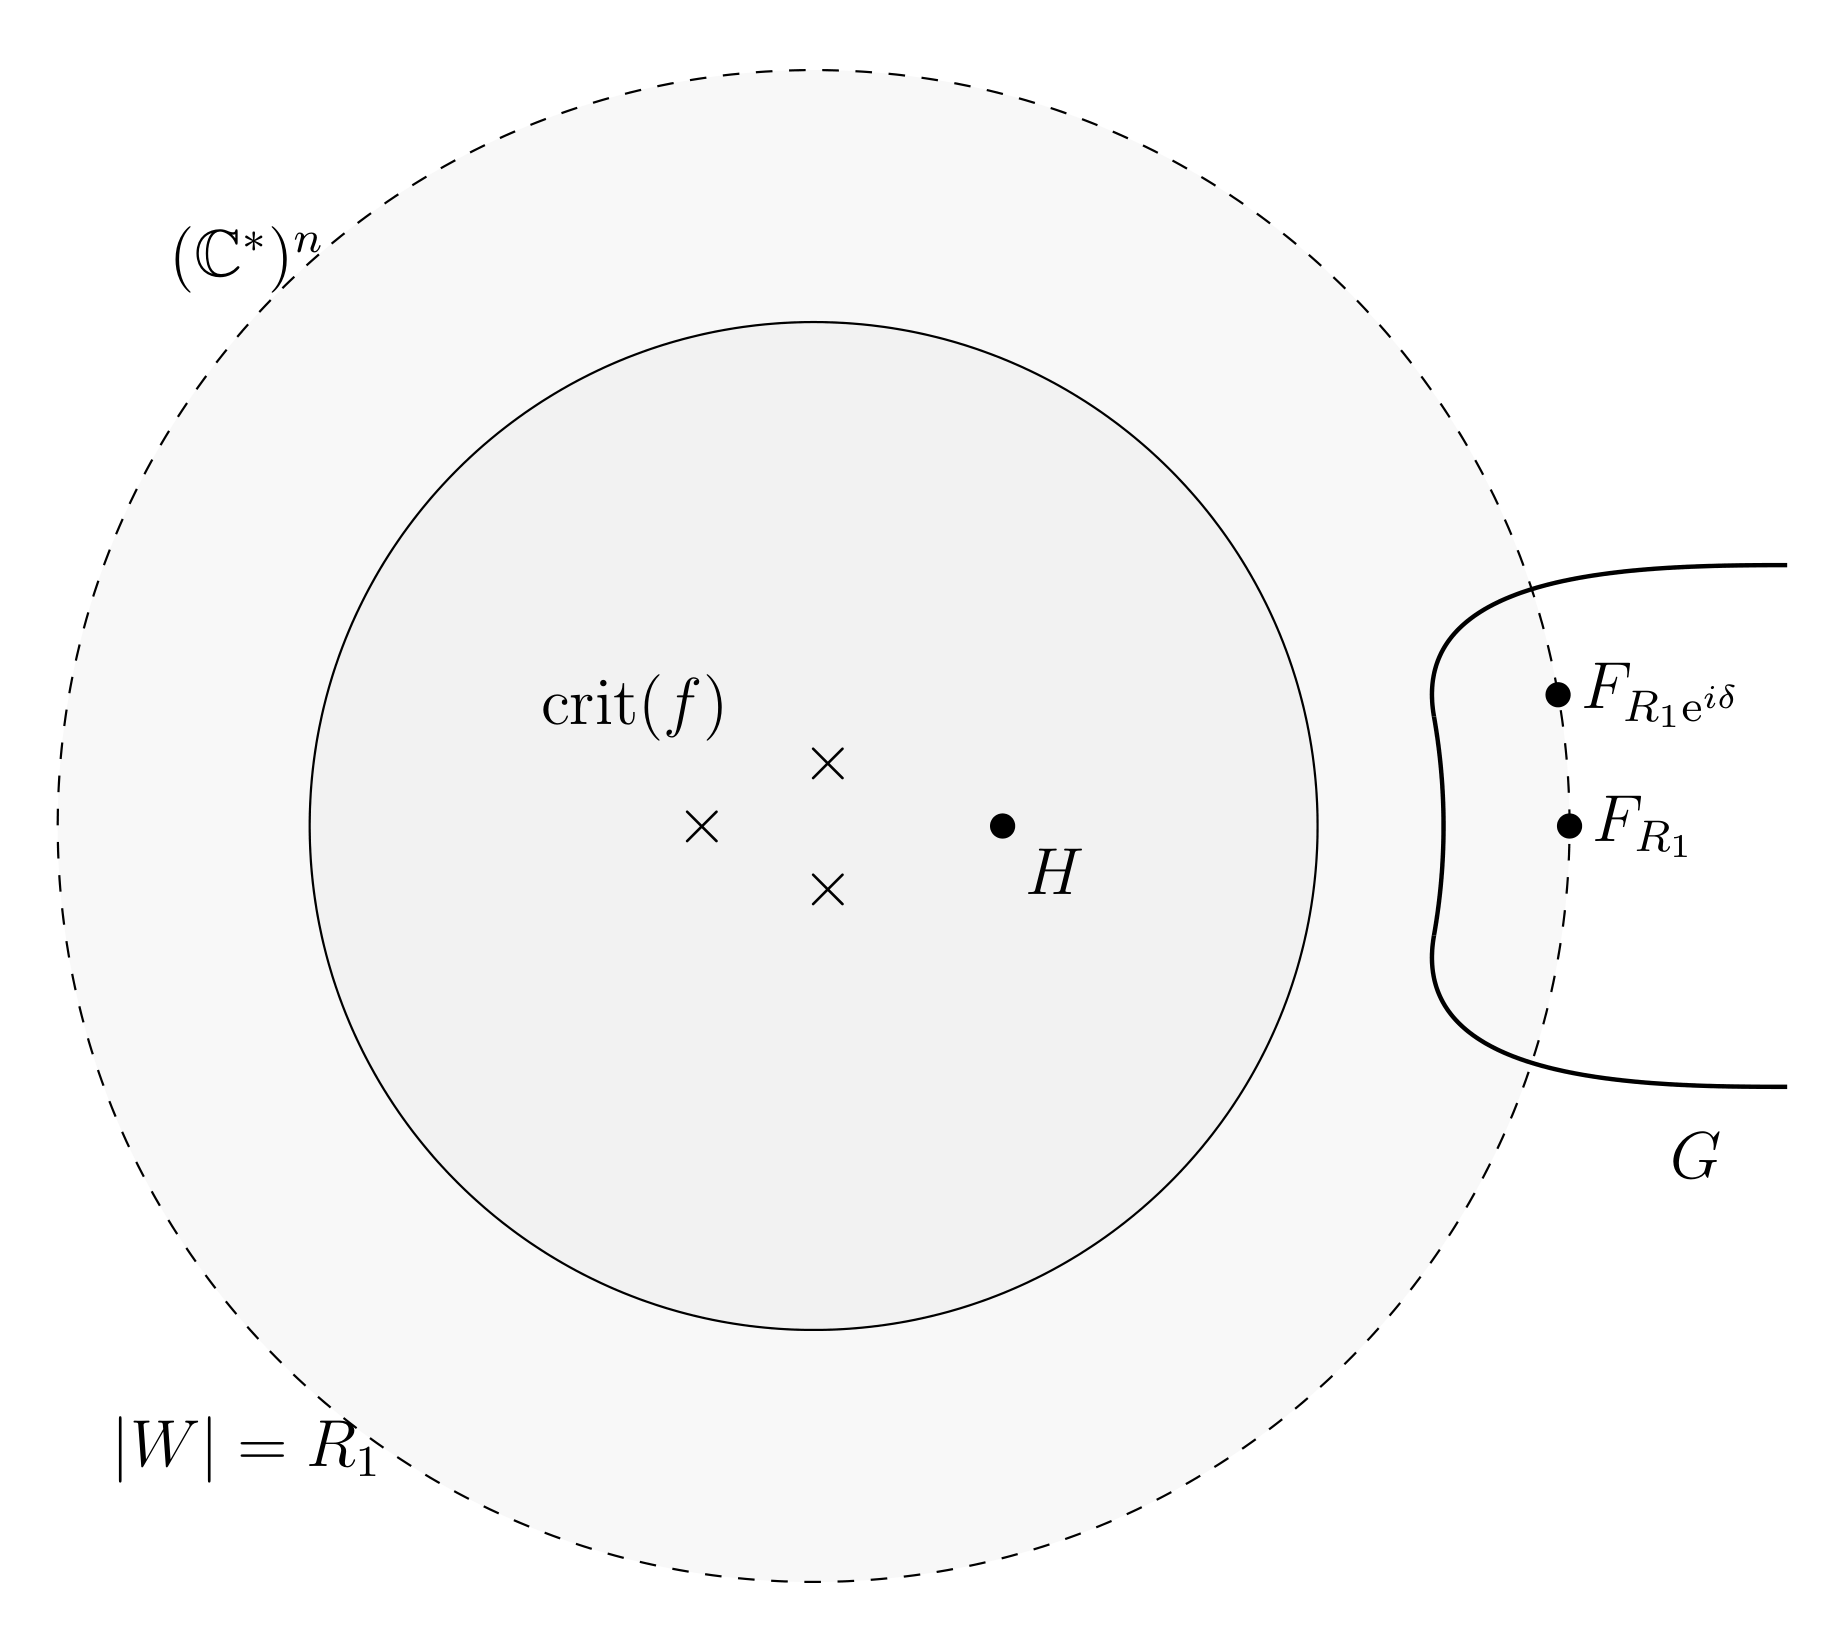
\includegraphics[width=0.54\textwidth]{figures/fig7_4.png}
\caption{命题 \ref{prop:7-1-2} 的证明：超曲面 $F_{R_1e^{i\delta}}$、$F_{R_1}$ 与扇形超曲面 $G$。}
\label{fig:7-4}
\end{figure}

% ===== 原书 p.103 =====
\begin{figure}[htbp]
\centering
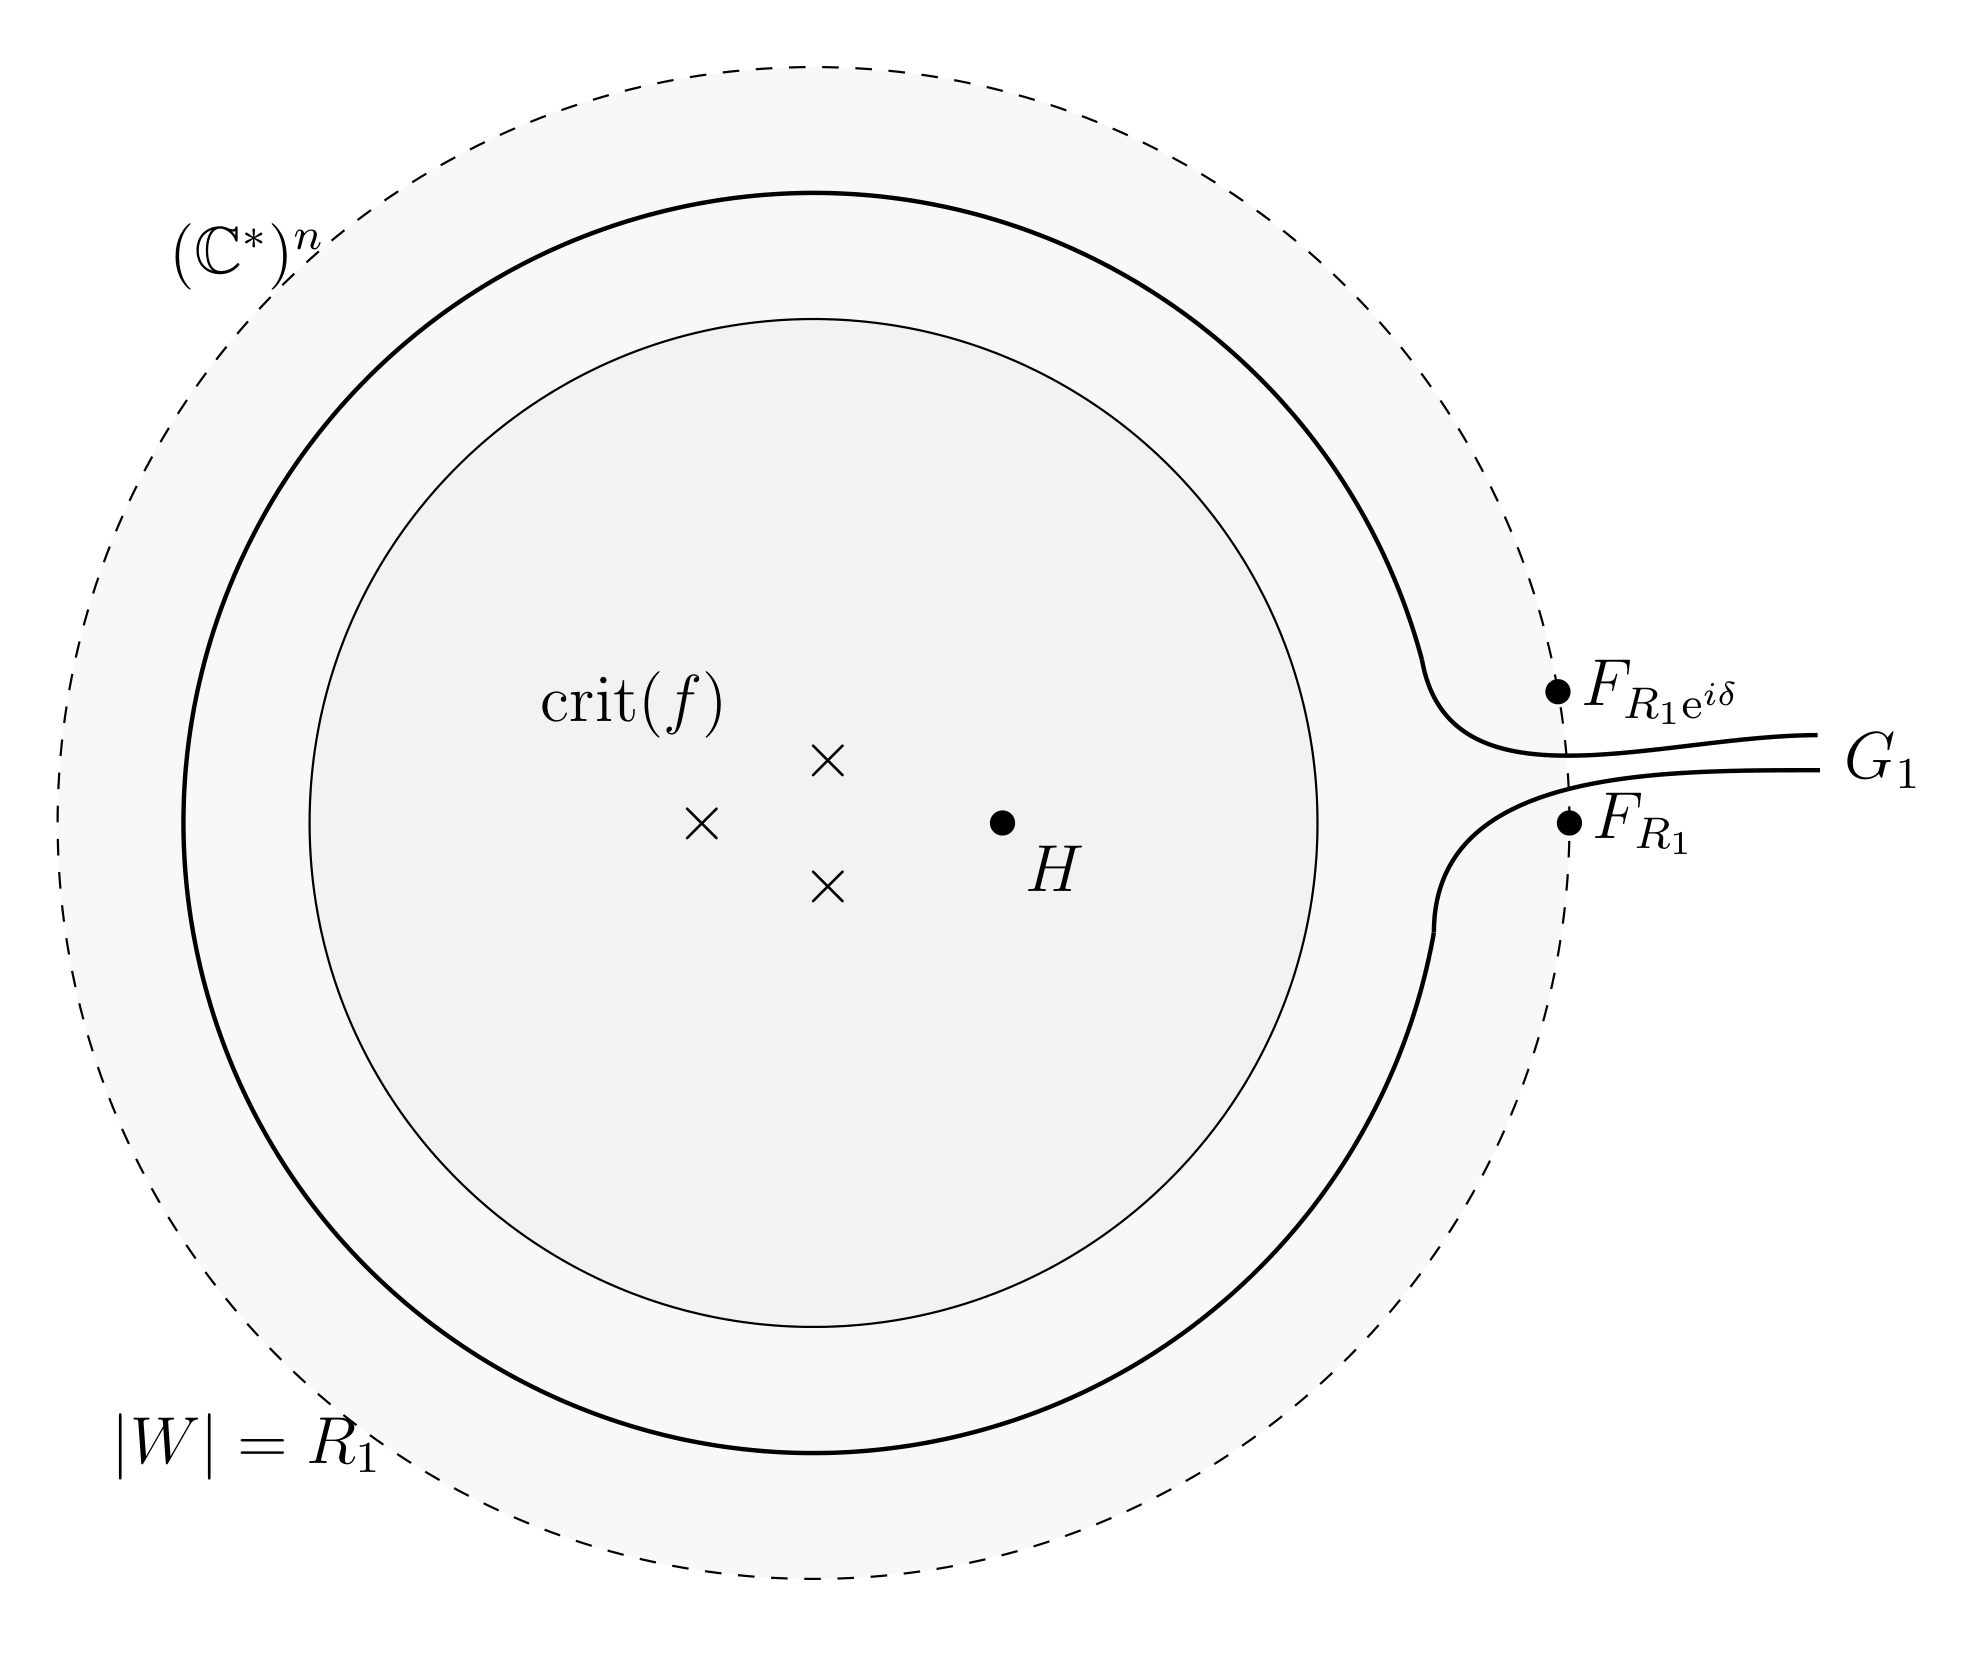
\includegraphics[width=0.54\textwidth]{figures/fig7_5.png}
\caption{命题 \ref{prop:7-1-2} 的证明：施加以 $F_{R_1e^{i\delta}}$ 与 $F_{R_1}$ 互换的同痕之后，扇形超曲面 $G$ 的像 $G_1$。}
\label{fig:7-5}
\end{figure}

% ===== 原书 p.104 =====
\item 作与 [Jef22, Proposition 6] 类似的论证：施加一个把被去掉的纤维移到无穷远的同痕，再应用 [GPS20a, Lemma 2.32] 的唯一性结果，可以证明 Liouville 扇形 $X_0=(\C^*)^n\cap\{\operatorname{Re}(z)\le0\}$ Liouville 同伦于如下结果：把 [Syl19b, Proposition 2.6] 应用于 Liouville 区域 $(\C^*)^n_0=\{|W|\le R_1\}\cap\{\psi\le R_2\}$，沿一对 Liouville 超曲面 $F=|W|^{-1}\bigl(\{R_1,R_1e^{i\delta}\}\bigr)\cap\{\psi\le R_2-\eps\}$ 切开。这里我们经 $\Phi_\eta$ 等同 $F_{R_1e^{i\delta}}$ 与 $F_{R_1}$。

等价地，取双覆盖 $q\colon\C\to\C$，使 $q(z)=c$ 的两个根在 $c$ 绕单位圆一周时描出曲线 $\gamma$ 与 $\eta(t)=e^{it\delta}$。令 $\tilde f(x)=q(1-f(x))$，则 Liouville 扇形 $(\C^*)^n\cap\{\operatorname{Re}(z)\le0\}\setminus\{0\}$ Liouville 同伦于：把 [Syl19b, Proposition 2.6] 应用于 Liouville 区域 $(\C^*)^n_0$ 与超曲面 $F=\tilde f^{-1}(1)\cap\{\phi\le R_2-\eps\}$ 的结果。

\transnote{易错预警：$(\C^*)^n_0$ 的下标 $0$ 指“取 $|W|\le R_1$ 截断后的区域”，与 $\eta_0$、$\alpha_0$、$\cW_0$ 的下标 $0$ 无关，切勿混为一谈。}

\item 由 [GPS20a, Lemma 2.32] 的同伦唯一性，取 Liouville 超曲面的同痕 $\widetilde F_t=\tilde f^{-1}(e^{2\pi it})$（$t\in[0,1]$），给出相应 Liouville 扇形 $X_t$ 的唯一 Liouville 同伦。扇形边界 $\partial X_1$ 的两个分支经 Liouville 流回缩（对应图 \ref{fig:7-3} 中标出的两个黑点）之后，与 $F_{R_1e^{i\delta}}\times\R$ 及 $F_{R_1}\times\R$ 典范等同。

此外，扇形超曲面 $G=\{\operatorname{Re}(z)=-\rho/2\}\subseteq X_0$ 会在该同伦下变为扇形超曲面 $G_t\subseteq X_t$，并在无穷远处保持平行于 Liouville 向量场：见图 \ref{fig:7-4}。这个扇形超曲面把 $X_t$ 表示成两个扇形的粘合；由唯一性引理，第一个 Liouville 同伦于 $((\C^*)^n,f)$，第二个 $X^t_{A_2}$ 同伦于 $H\times A_2$（见图 \ref{fig:7-6}）。

\transnote{含糊点拨：原文说 $X^t_{A_2}$ “同伦于 $H\times A_2$”，指 Liouville 同伦而非辛同胚；扇形 $X^t_{A_2}$ 随 $t$ 变动，只有同伦类保持不变。}

% ===== 原书 p.105 =====
\item 最后，把扇形 $H\times A_1$ 沿 $\partial X_1$ 粘到 $X_1$ 所得的结果，是一个 Liouville 同伦于 $(\C^*)^n\setminus H$ 的 Liouville 流形（见图 \ref{fig:7-6}）。我们来理解这一粘合涉及的等同。Liouville 同痕 $\widetilde F_t$ 给出辛同胚 $\Phi_\gamma\colon F_{R_1}\to H$ 与 $\Phi_\eta\colon F_{R_1e^{i\delta}}\to H$，它们把边界 $\partial X_1$ 表示成 $(H\times\R)\sqcup(H\times\R)$。

在原来的表示 $X_0$ 中，我们把 $X_{A_1}$ 粘到 $X_{A_2}$ 得到 $(\C^*)^n\setminus H$。回忆纤维 $F_{R_1}$ 经沿一条射线的平行移动与参考纤维 $H$ 等同。这条纤维 $F_{R_1}$ 是 [Syl19b, Proposition 2.6] 的形变之后 Liouville 流的源头，故 $((\C^*)^n,f)$、$X_{A_2}$ 与 $X_{A_1}$ 的扇形边界的每个分支都典范等同于 $F_{R_1}\times\R$。

于是，用原来的粘合映射 $\id\colon F_{R_1}\to F_{R_1}$ 与 $\Phi_\eta\colon F_{R_1}\to F_{R_1e^{i\delta}}$ 把 $X_{A_1}$ 粘回 $X_1$，再与我们已有的与 $H$ 的等同复合，就得到粘合映射 $\mu\colon H\to H$ 与 $\Phi_\eta\colon H\to H$（后者同痕于恒等）。这就完成了论断的证明。
\end{enumerate}
\end{proof}

\transnote{易错预警：此处的 $\mu\colon H\to H$ 是辛同胚（几何单值性），不是第 8 章讨论的单值函子 $\mu\colon\cW(H)\to\cW(H)$，也不是前面带停点范畴里的 $\mu$ 单子；同名不同物。}

\begin{remarkx}\label{rem:10}
我们应把这一分解看成与表示 $\tilde f_\infty=0$ 相联系的 $(\C^*)^n\setminus H$ 的扇形分解。此时改用 $-1/f$ 给出的投影 $(\C^*)^n\setminus H\to\C$。其效果是交换 $0$ 与 $\infty$：$f$ 的全部单值性现在都围绕 $0\in\C^*$ 发生。
\end{remarkx}

相应地，我们本想用超曲面 $\operatorname{Re}(1/f)=1/2$ 把 $(\C^*)^n\setminus H$ 切成两个扇形。技术细节使这一点难以实行，所以我们改用命题 \ref{prop:7-1-2} 给出的论证，得到一种等价的扇形粘合表示。第二作者与合作者未来的工作将去掉对这一论证的需要。

\transnote{背景直觉：把 $f$ 换成 $-1/f$ 是“交换零与无穷”的标准手法：$f$ 的奇异纤维位于 $0$ 上方，$-1/f$ 的奇异纤维则跑到无穷远，同时单值性挪到 $0\in\C^*$ 附近。}

\begin{definition}\label{def:7-1-3}
给定上述扇形分解，我们定义：
\begin{enumerate}
\item 函子 $\alpha_\infty\colon\cW((\C^*)^n,f)\to\cW((\C^*)^n\setminus H)$ 由命题 \ref{prop:7-1-1} 中的扇形包含给出；
\item 函子 $\alpha_0\colon\cW((\C^*)^n,f)\to\cW((\C^*)^n\setminus H)$ 由命题 \ref{prop:7-1-2} 中的扇形包含给出。
\end{enumerate}
\end{definition}

% ===== 原书 p.106 =====
\begin{figure}[htbp]
\centering
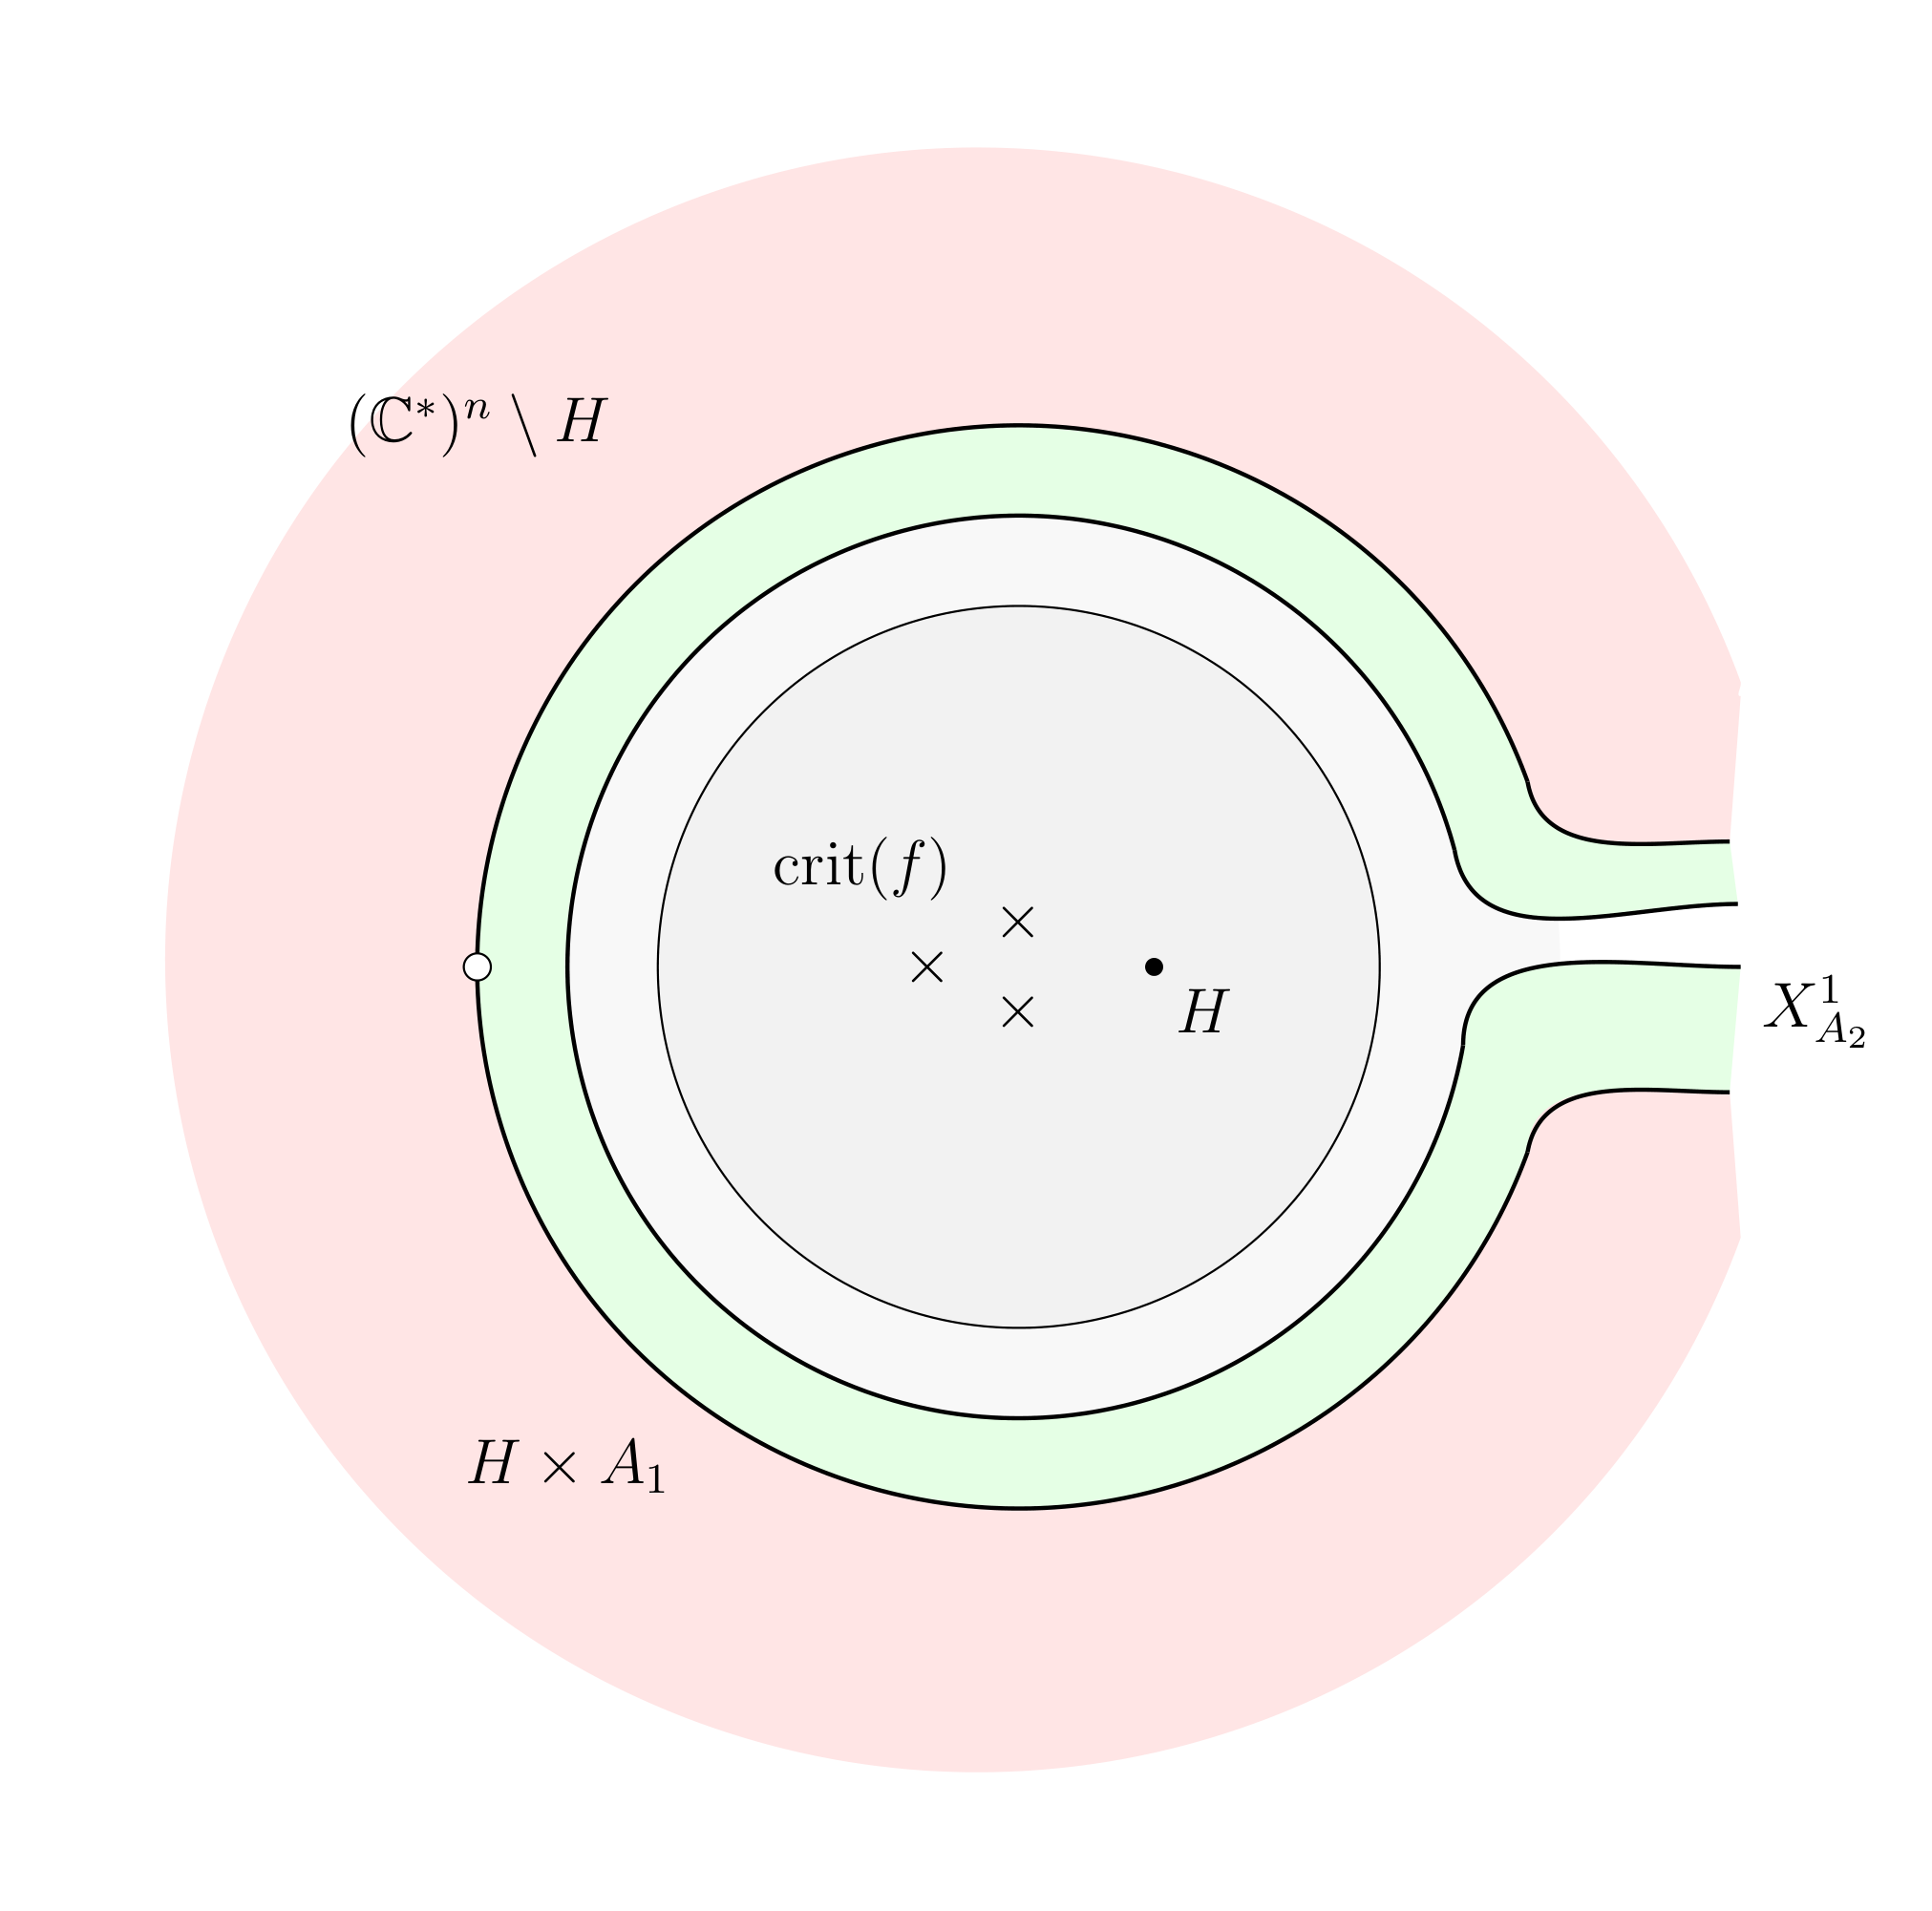
\includegraphics[width=0.55\textwidth]{figures/fig7_6.png}
\caption{命题 \ref{prop:7-1-2} 的证明：扇形 $X^1_{A_2}$ 为绿色，扇形 $H\times A_1$ 为红色。}
\label{fig:7-6}
\end{figure}

% ===== 原书 p.107 =====
\begin{corollary}\label{cor:7-1-4}
有 wrapped Fukaya 范畴的推出（pushout）图表：
\[
\begin{tikzcd}[column sep=3.0em, row sep=1.8em]
\cW(H) \arrow[r, "\cup"] \arrow[d] & \cW((\C^*)^n,f) \arrow[d, "\alpha_\infty"] \\
\cW(H\times\C^*(2),z) \arrow[r] & \cW_0((\C^*)^n\setminus H)
\end{tikzcd}
\qquad
\begin{tikzcd}[column sep=3.0em, row sep=1.8em]
\cW(H) \arrow[r, "\cup"] \arrow[d] & \cW((\C^*)^n,f) \arrow[d, "\alpha_0"] \\
\cW(E,z) \arrow[r] & \cW_\infty((\C^*)^n\setminus H)
\end{tikzcd}
\]
其中 $\cW(H\times\C^*(2),z)$ 记如下 wrapped Fukaya 范畴：简单逆时针 Reeb 轨道绕 $0$ 的次数为 $2$。
\end{corollary}

\transnote{易错预警：$\C^*(2)$ 里的 $(2)$ 是分次移位的信息，不是幂次，也不是“取两次”的记号；它表示绕 $0$ 的简单逆时针 Reeb 轨道的次数为 2。}

\begin{proof}
见 [GPS19, Theorem 1.28]：检查其论证可知，只要分次数据适当地粘合，那些论证可推广到 $\Z$-分次范畴（参 [GPS20c]）。注意 $\eta_0$ 由 $\eta_\infty$ 作上同调类 $[\arg(f)]$ 的扭得到；该上同调类限制到子扇形 $((\C^*)^n,f)$ 上平凡（因为 $f$ 在那里作为 Cartier 除子平凡），所以两个图表中可以使用同一个 $\Z$-分次范畴 $\cW((\C^*)^n,f)$。
\end{proof}

\begin{remarkx}\label{rem:11}
注意这些几何粘合结果与所选的分次结构无关；因此上面两个图既可以写成用 $\eta_0$-分次，也可以写成用 $\eta_\infty$-分次。
\end{remarkx}

\subsection{镜像对称}

\begin{proposition}\label{prop:7-2-1}
有交换图表：
\[
\begin{tikzcd}[column sep=4.4em, row sep=2.8em]
\cW(H) \arrow[r] \arrow[d, "\cup"'] & \operatorname{Coh}(D) \arrow[d, "i_{D*}"] \\
\cW((\C^*)^n,f) \arrow[r] & \operatorname{Coh}(X)
\end{tikzcd}
\]
其中横箭头是 [GS22; Kuw20] 给出的等价。此外，$f$ 绕 $\infty$ 的逆时针单值函子 $\mu\colon\cW(H)\to\cW(H)$ 镜像于 $\operatorname{Coh}(D)$ 上与反典范丛 $\cK_X^{-1}|_D$ 作张量。
\end{proposition}

\transnote{易错预警：原图在竖箭头旁另画弧形箭头，表示左伴随：$\cup$ 的左伴随是 $\cap$，$i_{D*}$ 的左伴随是 $i_D^*$。这两个伴随在证明中被用来把一侧的等价搬到另一侧，读图时不可略去。}

\begin{proof}
我们知道，在 [GS22] 的镜像对称等价下 $\cup$ 与 $i_{D*}$ 相对应（见 Figure 6）。因此它们的左伴随 $\cap^L$ 与 $i_D^*$ 也必定互为镜像。用反常束的语言说，球函子 $S$ 的对偶余扭（dual cotwist）由余单位映射 $S^LS\to\id$ 的锥给出，其中 $S^L$ 记左伴随。

[Syl19d, Theorem 1.3] 证明：$f$ 绕 $\infty$ 的几何逆时针单值性 $\mu$ 作用在 $\cW(H)$ 上时，等于 $\cup$ 的对偶余扭再平移 $[2]$。由 [Nad19b, p.12] 可知，$i_{D*}$ 的对偶余扭由 $\otimes\cK_X^{-1}|_D[-2]$ 给出。消去这两个 2-平移，即知函子 $\mu$ 对应于 $\otimes\cK_X^{-1}|_D$。
\end{proof}

\transnote{含糊点拨：原文作“见 Figure 6”，指原书第 6 章的图 6。本译注把第 6 章编为另一块，此处照原文字面译出，未加交叉引用。}

\begin{proposition}\label{prop:7-2-2}
$(E,H)$ 与 $K_X|_D$ 之间存在镜像对称等价，使得下图交换：
\[
\begin{tikzcd}[column sep=3.6em, row sep=2.2em]
\cW(H) \arrow[r] \arrow[d, "\cup"'] & \operatorname{Coh}(D) \arrow[d, "\iota_{D*}"] \\
\cW(E,z) \arrow[r] & \operatorname{Coh}(K_X|_D)
\end{tikzcd}
\]
其中顶部横箭头是 [GS22] 的等价。
\end{proposition}

% ===== 原书 p.108 =====
\begin{proof}
$K_X|_D$ 的全空间是 $D$ 上代数层 $\operatorname{Sym}(\cK_X^{-1}|_D)$ 的相对 Spec。于是全空间上的相干层范畴，由 $D$ 上带相干 $\operatorname{Sym}(\cK_X^{-1}|_D)$-模结构的拟相干层 $\mathcal F$ 构成的范畴给出。由 $\operatorname{Sym}$ 的泛性质，这样的数据等同于一个态射 $\mathcal F\otimes\cK_X^{-1}|_D\to\mathcal F$，它描述 $\operatorname{Sym}(\cK_X^{-1}|_D)$ 的生成元如何作用在 $\mathcal F$ 的截面上。

因此可以把 $\operatorname{Coh}(K_X|_D)$ 描述为如下对 $(\mathcal F,\varphi\colon\mathcal F\otimes\cK_X^{-1}|_D\to\mathcal F)$ 的范畴：$\mathcal F$ 是 $D$ 上的拟相干层，$\varphi$ 使 $\mathcal F$ 具有 $(\cdot\otimes\cK_X^{-1}|_D)$-单子上的有限生成模结构。参 [Gam20, Proposition 5.8]。推前函子 $\operatorname{Coh}(D)\to\operatorname{Coh}(K_X|_D)$ 只是把层 $\mathcal F$ 送到平凡作用 $\mathcal F\otimes\cK_X^{-1}|_D\to\mathcal F$。

\transnote{含糊点拨：“相对 Spec”指把 $\operatorname{Sym}(\cK_X^{-1}|_D)$ 看作 $D$ 上的拟凝聚代数层，再取它在 $D$ 上的相对谱；$K_X|_D$ 作为 $D$ 上的线丛，其全空间正是这个相对 Spec。}

% ===== 原书 p.109 =====
对 $\cW(E,H)$ 有类似的描述：引理 \ref{prop:7-1-2} 中的扇形分解把 $\cW(E,H)$ 表示成 wrapped Fukaya 范畴的同伦余极限。注意：尽管我们用的是 $1-f$ 而不是 $f$，平行移动 $\mu$ 仍自然同构于几何逆时针单值函子。这可以用 [GPS19, A.4] 的显式同伦余极限构造实现：$\cW(E,H)$ 由对 $(L,s\colon\mu L\to L)$ 的范畴给出，其中 $L$ 是 $\cW(H)$ 上的模，$s$ 是使 $L$ 具有 $\mu$ 单子上的有限生成模结构的态射。此外，cup 函子 $\cW(H)\to\cW(E,H)$ 把拉格朗日量 $L$ 送到零态射 $\mu L\to L$。

把这些对 $\cW(E,H)$ 与 $\operatorname{Coh}(K_X|_D)$ 的描述与命题 \ref{prop:7-2-1} 结合，即得结论。
\end{proof}

\transnote{易错预警：原书此处写“引理”并附编号 7.1.2，但该编号实际对应命题；据上下文（扇形分解给出 $\cW(E,H)$ 的同伦余极限）应指该命题。译文按原文字面保留“引理”一词，交叉引用指向命题 \ref{prop:7-1-2}。}

\begin{proposition}\label{prop:7-2-3}
有范畴的推出图表：
\[
\begin{tikzcd}[column sep=2.6em, row sep=1.8em]
\operatorname{Coh}(D) \arrow[r, "i_{D*}"] \arrow[d, "\iota_{\tilde D*}"'] & \operatorname{Coh}(X) \arrow[d] \\
\operatorname{Coh}(D\times\mathbb A^1[-1]) \arrow[r] & \operatorname{Coh}(\tilde Z)
\end{tikzcd}
\qquad
\begin{tikzcd}[column sep=2.6em, row sep=1.8em]
\operatorname{Coh}(D) \arrow[r, "i_{D*}"] \arrow[d, "\iota_{D*}"'] & \operatorname{Coh}(X) \arrow[d] \\
\operatorname{Coh}(K_X|_D) \arrow[r] & \operatorname{Coh}(Z)
\end{tikzcd}
\]
其中 $\operatorname{Coh}(\tilde Z)$ 记导出概型 $\tilde Z$ 上相干层的范畴。
\end{proposition}

% ===== 原书 p.110 =====
\begin{proof}
由导出概型上 ind-coherent 层（ind-coherent sheaf）的真下降（见 [GR17, Proposition 7.2.2]）并取紧对象即得。
\end{proof}

\begin{theorem}\label{thm:7-2-4}
在选取由上述推出图表诱导的适当镜像等价之后：
\begin{enumerate}
\item $\cW_0((\C^*)^n\setminus H)$ 与 $\operatorname{Coh}(\tilde Z)$ 之间存在范畴等价，使函子 $\alpha_\infty$ 镜像于 $i_{\tilde X*}$；
\item $\cW_\infty((\C^*)^n\setminus H)$ 与 $\operatorname{Coh}(Z)$ 之间存在范畴等价，使函子 $\alpha_0$ 镜像于 $i_{X*}$。
\end{enumerate}
\end{theorem}

\begin{proof}
由命题 \ref{prop:7-2-1} 与 \ref{prop:7-2-2}，[GS22] 的镜像等价把推论 \ref{cor:7-1-4} 的 cup 函子与命题 \ref{prop:7-2-3} 中相干层上的推前函子交错对应。因此存在推出范畴 $\cW_0((\C^*)^n\setminus H)$ 与 $\operatorname{Coh}(\tilde Z)$ 之间的等价，以及 $\cW_\infty((\C^*)^n\setminus H)$ 与 $\operatorname{Coh}(Z)$ 之间的等价，使下图交换。
\end{proof}

\[
\begin{tikzcd}[column sep=1.4em, row sep=1.6em]
\operatorname{Coh}(D) \arrow[rrrr, "\iota_{\tilde D*}"] \arrow[dd, "i_{D*}"'] & & & & \operatorname{Coh}(D\times\mathbb A^1[-1]) \arrow[dd, "j_{\tilde D*}"'] \\
& \cW(H) \arrow[rr, "\cup"] \arrow[dd, "\cup"'] \arrow[ul, "\sim"'] & & \cW(H\times\C^*(2),z) \arrow[ur, "\sim"'] \arrow[dd] & \\
\operatorname{Coh}(X) \arrow[rrrr, "i_{\tilde X*}"] & & & & \operatorname{Coh}(\tilde Z) \\
& \cW((\C^*)^n,f) \arrow[rr, "\alpha_\infty"'] \arrow[ul, "\sim"'] & & \cW_0((\C^*)^n\setminus H) \arrow[ur, "\sim"'] &
\end{tikzcd}
\]

\transnote{易错预警：图中 $\cW(H\times\C^*(2),z)\to\cW_0((\C^*)^n\setminus H)$ 这条竖直箭头没有标注；它就是推论 \ref{cor:7-1-4} 第一个推出图的下方横箭头，并非遗漏。}

% ===== 原书 p.111 =====
\[
\begin{tikzcd}[column sep=1.4em, row sep=1.6em]
\operatorname{Coh}(D) \arrow[rrrr, "\iota_{D*}"] \arrow[dd, "i_{D*}"'] & & & & \operatorname{Coh}(K_X|_D) \arrow[dd, "j_{D*}"'] \\
& \cW(H) \arrow[rr, "\cup"] \arrow[dd, "\cup"'] \arrow[ul, "\sim"'] & & \cW(E,H) \arrow[ur, "\sim"'] \arrow[dd] & \\
\operatorname{Coh}(X) \arrow[rrrr, "i_{X*}"] & & & & \operatorname{Coh}(Z) \\
& \cW((\C^*)^n,f) \arrow[rr, "\alpha_0"'] \arrow[ul, "\sim"'] & & \cW_\infty((\C^*)^n\setminus H) \arrow[ur, "\sim"'] &
\end{tikzcd}
\]

\begin{remarkx}\label{rem:12}
定理 \ref{thm:7-2-4} 之所以这样陈述，是因为所给的论证并未证明：这些推出图表诱导的 $\cW((\C^*)^n\setminus H)$ 与 $\operatorname{Coh}(Z)$ 之间的镜像对称等价，必定与来自 [GS22] 的等价相同（尽管实际上它们确实相同）。
\end{remarkx}

\begin{remarkx}\label{rem:13}
不能通过把拉格朗日量送到自身来构造函子 $\cW_0((\C^*)^n\setminus H)\to\cW_\infty((\C^*)^n\setminus H)$，因为拉格朗日量未必对两种分次同时具有分次提升。即使限制到对两者都有分次的拉格朗日量子范畴，在对象与态射上取恒等的函子也不是 $\Z$-分次的，而只是 $\Z/2$-分次范畴上的函子。

同样地，$\operatorname{Coh}(Z)\to\operatorname{Coh}(\tilde Z)$ 似乎存在一个显然的函子，但应当使用的正确 $\Z$-分次等价由 Kn{\"o}rrer 周期性中介。A 侧相应的等价可以非正式地理解为在底空间里作变换 $z\mapsto1/z$。
\end{remarkx}

\transnote{易错预警：$\Z$-分次与 $\Z/2$-分次是本题的关口：对象层面恒等的函子会丢掉分次信息，因此只能在 $\Z/2$-分次范畴上成为函子；若要拿到 $\Z$-分次等价，必须借 Kn{\"o}rrer 周期性。}
